\chapter[Resultados Alcançados]{Resultados Alcançados}\label{cap4}


O Editor de \textit{audiobooks} gera com sucesso um formato Ogg Vorbis com todos os metadados inseridos no pacote Vorbis de comentários e as marcações de conteúdo contidas no pacote LGMK construído. Mesmo com sua estrutura alterada, o formato *.ogg pode ser executado em players com suporte a arquivos como o \textit{sox} ou Rhythmbox.

A efeito de comparação ao \cite{herbert}, cujo trabalho desenvolveu um formato parecido que não faz uso da compressão de dados, também foi utilizado o Hino Nacional Brasileiro para simular um \textit{audiobook}. O arquivo original no formato WAV possui 3 minutos e 41 segundos de duração e ocupa 42,5 MB de espaço em memória. Este arquivo foi carregado pelo Editor e em seguida foram inseridos os mesmos metadados inseridos por \cite{herbert} conforme mostra Tabela \ref{tab1}.

\begin{table}[ht]
\centering
\caption{Metadados inseridos no \textit{comment header}.}
\vspace{0.5cm}
\begin{tabular}{ll}

\hline
\textbf{Nome} & \textbf{Valor} \\
\hline
Título & Hino Nacional Brasileiro \\
Autor & Joaquim Osório \& Francisco Manuel \\
Idioma & Português \\
Editora & \\
Local de Criação & Brasil \\
Número de Páginas & 0 \\
Ano de Criação & 1822 \\
\hline

\end{tabular}
\label{tab1}
\end{table}

Para verificarmos os metadados inseridos no pacote de comentários do formato Ogg, a Figura \ref{meta}

 \begin{figure}[ht]
	\centering
		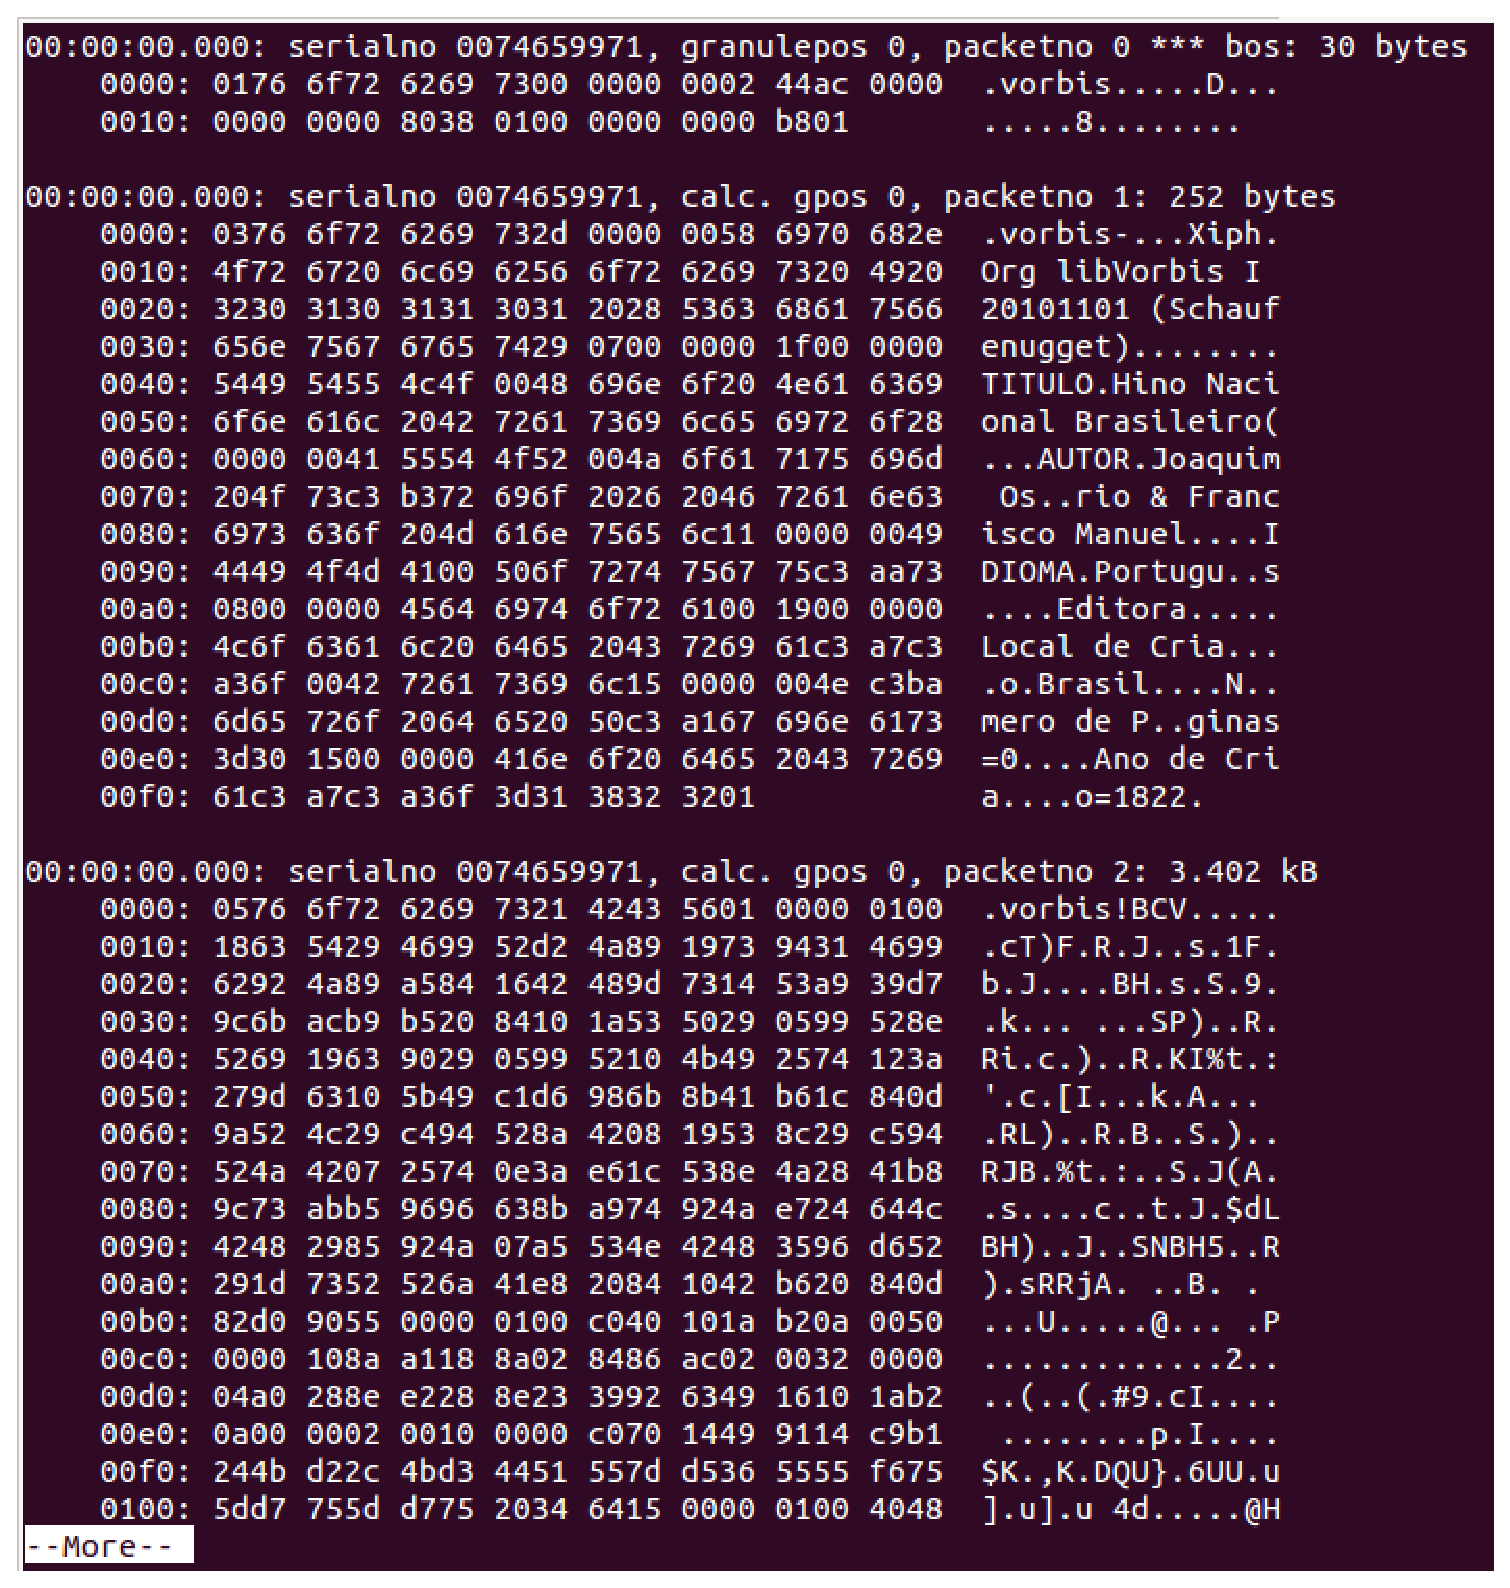
\includegraphics[keepaspectratio=true,scale=0.3]{figuras/hnbogg.eps}
	\caption{Utilização do oggz-dump - pacote de comentários.}
	\label{meta}
\end{figure}

O pacote de comentários é o pacote número 1 e pode-se perceber que os metadados foram inseridos corretamente. Relacinado as marcações de conteúdo,  a Tabela \ref{mark} mostram as informações que serão inseridas no pacote LGMK. As marcações também foram as mesmas utilizadas por \cite{herbert}.

\begin{table}[ht]
\centering
\caption{Marcações inseridas no \textit{LGMK header}.}
\vspace{0.5cm}
%\rowcolor{1}{}{lightgray}
\begin{tabular}{ll}

\hline
\textbf{Nome da Marcação} & \textbf{Tempo(s)} \\
\hline
Parte 1 & 0 \\
Parte 2 & 103 \\
Introdução 1 & 0 \\
Primeira Estrofe & 28 \\
Segunda Estrofe & 44 \\
Terceira Estrofe & 60 \\
Quarta Estrofe & 64 \\
Quinta Estrofe & 79 \\
Sexta Estrofe & 91 \\
Introdução 2 & 103 \\
Sétima Estrofe & 132 \\
Oitava Estrofe & 148 \\
Nona Estrofe & 164 \\
Décima Estrofe & 168 \\
Décima Primeira Estrofe & 183 \\
Décima Segunda Estrofe & 195 \\
Décima Terceira Estrofe & 201 \\
Final & 206 \\
\hline

\end{tabular}
\label{mark}
\end{table}

O verificação da inserção dos marcadores de conteúdo no pacote LGMK pode ser visualizado usando a ferramenta oggz-dump. A Figura \ref{lgmk} mostra o pacote LGMK que pode ser identificado pelo número de pacote 3 e os marcadores de conteúdo contidos dentro dele.

 \begin{figure}[ht]
	\centering
		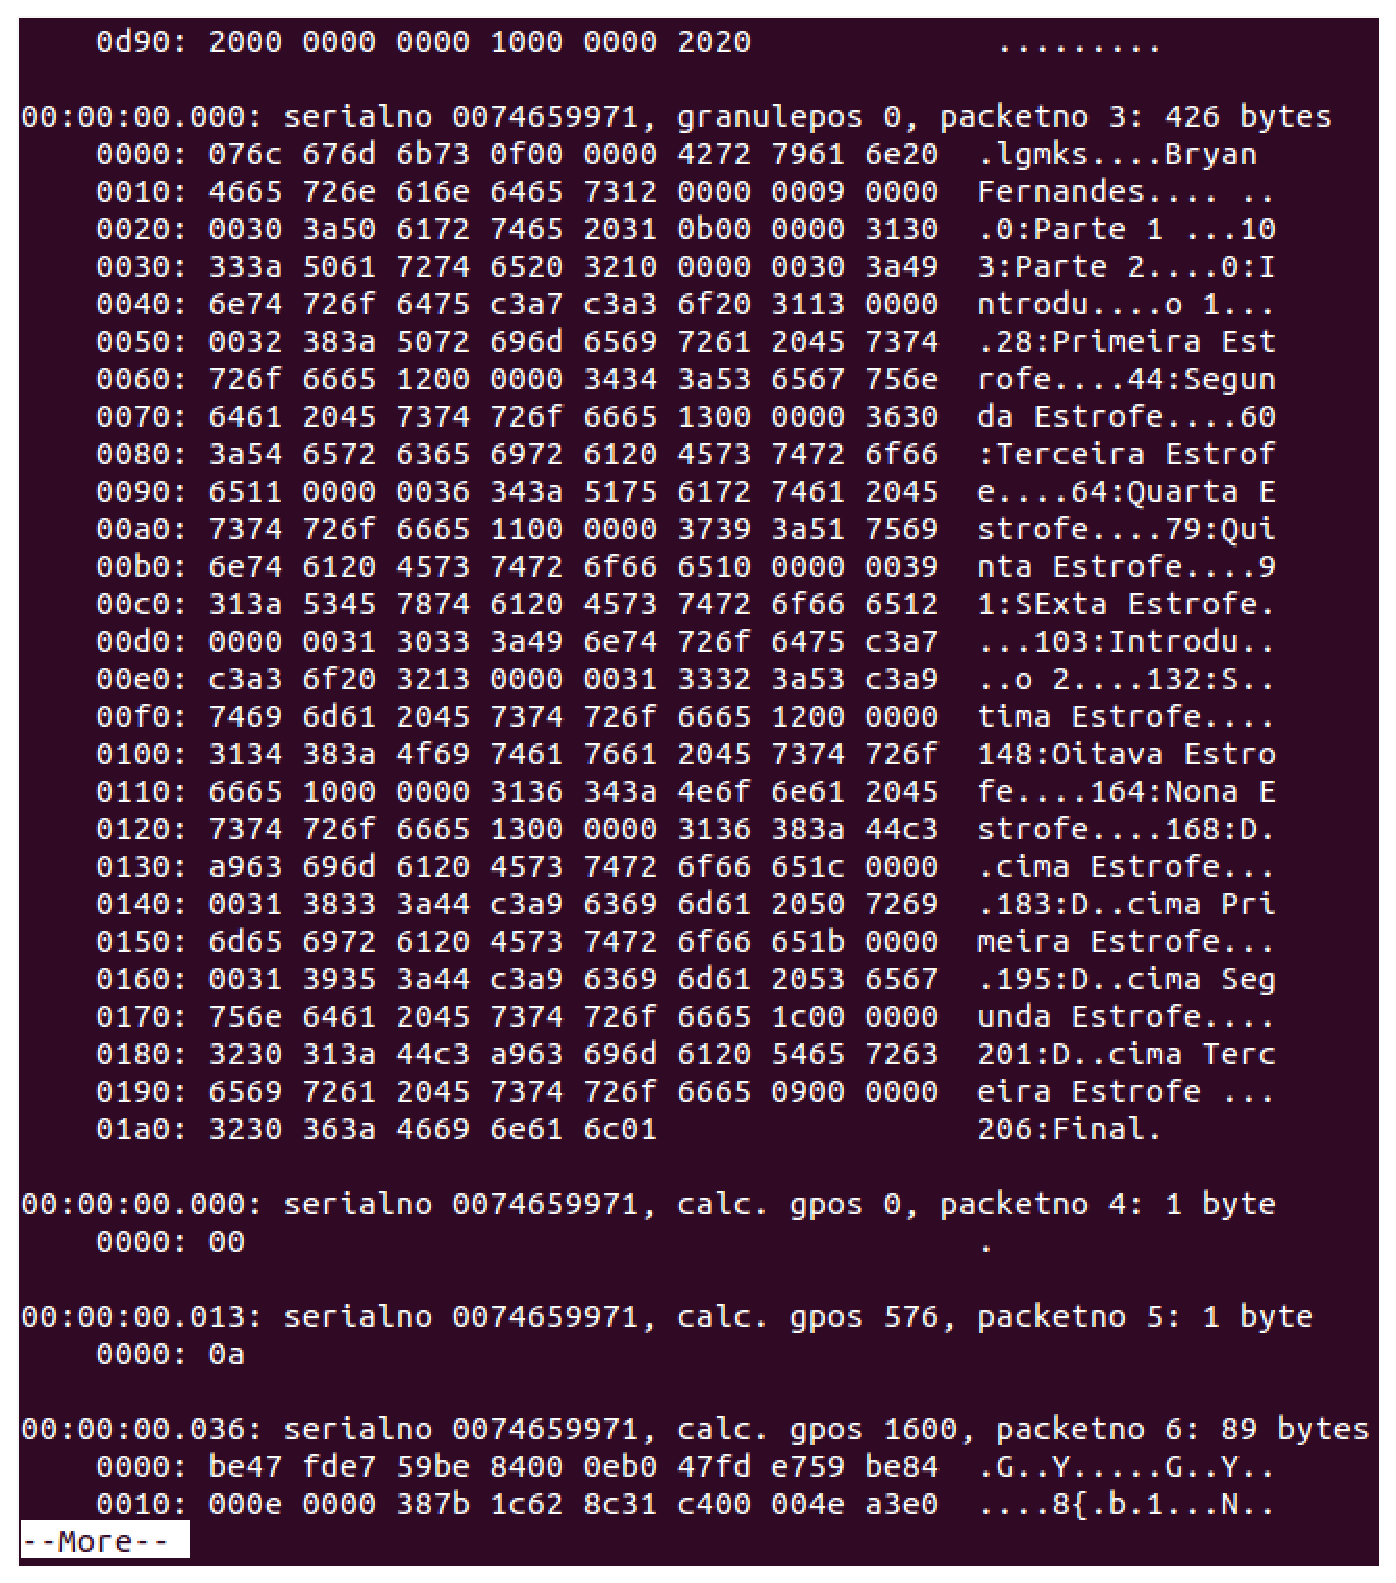
\includegraphics[keepaspectratio=true,scale=0.3]{figuras/hnblgmkogg.eps}
	\caption{Utilização do oggz-dump - pacote LGMK.}
	\label{lgmk}
\end{figure}

O pacote Ogg Vorbis gerado possui apenas 1,84MB e não mais 42,5MB como o arquivo original. Houve uma redução considerável devido ao algoritmo de compressão do \textit{codec} Vorbis. O arquivo gerado é executado corretamente do início ao fim sem interrupções. Também foi feito um teste para verificar se o pacote LGMK não iria corromper o arquivo Ogg Voribs inserido 22 milhões de marcações. O arquivo final ficou com 340MB de tamanho, no entanto, o player conseguiu executá-lo normalmente.


%O Editor também é capaz de decodificar todos os dados conforme mostra a Figura \ref{decodeog%g}%
%
% \begin{figure}[ht]
%	\centering
%		\includegraphics[keepaspectratio=true,scale=0.5]{figuras/decodeogg.eps}
%	\caption{Utilização do Editor para decodificar os dados.}
%	\label{decodeogg}
%\end{figure}




%1,86MB

O Player desenvolvido é capaz de executar o novo formato gerado pelo Editor, e através das marcações contidas no formato, navegar pelo conteúdo do áudio facilmente. O uso Player não se dá apenas pela interface gráfica através do uso do mouse, pleo teclado também somos capazes de utilizar o player por meio das funções básicas de play/pause e de navegação utilizando as teclas direcionais. O Player está representado na Figura \ref{player}:

 \begin{figure}[ht]
	\centering
		\includegraphics[keepaspectratio=true,scale=0.5]{figuras/player.eps}
	\caption{Execução de um arquivo de teste gerado pelo Editor.}
	\label{player}
\end{figure}

O Player carrega os metadados referente ao arquivo informando ao usuário sobre qual arquivo está sendo executado bem como a visualização da posição em que o player se encontra no áudio gravado. Os comandos pelo teclado estão descritos abaixo:

\begin{itemize}
	\item{\textbf{Play/Pause}:} o comando pode ser executado alternativamente pela tecla de espaço;
	\item{\textbf{Pular uma marcação a frente}:} esta funcionalidade do player pode ser acionada através da tecla de seta para a direita;
	\item{\textbf{Voltar uma marcação}:} esta funcionalidade do player pode ser acionada através da tecla de seta para a esquerda;
	\item{\textbf{Subir a marcação para o nível 1}:} o comando pode ser acionado quando pressionada a tecla de seta para cima. Esta funcionalidade foi pensada com o intuito de contemplar a referência de capítulos contidas nos livros impressos;
	\item{\textbf{Descer a marcação para o nível 2}:} esta funcionalidade do player pode ser acionada através da tecla de seta para a baixo. Esta funcionalidade do player visa contemplar a referência para os subcapítulos como encontrado nos livros impressos, tornando a busca de informação ainda mais otimizada.
\end{itemize}

O Player foi testados nos sistemas operacionais Ubuntu e Mac OS X. Nos dois ambientes o player não apresentou nenhum erro durante a sua execução. Vale ressaltar que o Editor também é funcional netes dois sistemas operacionais.
